\documentclass[a4paper]{article}

\usepackage{INTERSPEECH2020}
\usepackage{cite}
\usepackage{tablefootnote}
\usepackage{color}
\usepackage{pifont}
\usepackage{footnote}
\makesavenoteenv{tabular}

\usepackage{soul}
\title{Unsupervised Subword Modeling Using Autoregressive Pretraining and Cross-Lingual Phone-Aware Modeling}
\name{Siyuan Feng, Odette Scharenborg}
%The maximum number of authors in the author list is twenty. If the number of contributing authors is more than twenty, they should be listed in a footnote or in acknowledgement section, as appropriate.
\address{
  Multimedia Computing Group, Delft University of Technology,  The Netherlands}% \\
 %$^2$Department of Electronic Engineering, The Chinese University of Hong Kong, Hong Kong}
\email{\{S.Feng, O.E.Scharenborg\}@tudelft.nl}

\begin{document}

\maketitle
% 
\begin{abstract}
  For your paper to be published in the conference proceedings, you must use this document as both an instruction set and as a template into which you can type your own text. If your paper does not conform to the required format, you will be asked to fix it.
  Please do not reuse your past papers as a template. To prepare your paper for submission, please always download a fresh copy of this template from the conference website and please read the format instructions in this template before you use it for your paper.
  Conversion to PDF may cause problems in the resulting PDF or expose problems in your source document. Before submitting your final paper in PDF, check that the format in your paper PDF conforms to this template. Specifically, check the appearance of the title and author block, the appearance of section headings, document margins, column width, column spacing, and other features such as figure numbers, table numbers and equation number. In summary, you must proofread your final paper in PDF before submission.
    The maximum number of pages is 5. The 5\textsuperscript{th} page may be used exclusively for references. 
    % The references should begin on an earlier page immediately after the Acknowledgements section, and continue onto the 5\textsuperscript{th} page. If no space is available on an earlier page, then the references may begin on the 5\textsuperscript{th} page.

%   Index terms should be included as shown below.
\end{abstract}
\noindent\textbf{Index Terms}: speech recognition, human-computer interaction, computational paralinguistics

\section{Introduction}

% Automatic speech recognition (ASR) has achieved impressive performance in recent years for major languages such as English \cite{Han2019State,Wang2019Transformer}.
% , thanks to the successful application of deep neural networks (DNNs) in acoustic and language modeling. 
% Acoustic modeling is a core component in building an ASR system. 
% It is   considered a supervised learning problem.  
Training a DNN acoustic model (AM) for a high-performance automatic speech recognition (ASR) system requires a huge amount of speech data paired with their corresponding transcriptions. 
%While this is considered not a problem for  languages such as English and Mandarin, 
Many languages in the world have very limited or even no transcribed data \cite{dunbar2017zero}. 
% In an extreme scenario where there are no transcribed data available for the concerned  language, 
% these languages are usually referred to as \textit{low-resource} languages. C
Conventional supervised acoustic modeling techniques are thus problematic or even not applicable to these languages.
% to low-resource languages.

Unsupervised acoustic modeling refers to the topic of modeling basic acoustic units of a language with only untranscribed speech available. It is a challenging topic with significant research impacts. It has been studied in applications to languages without orthographic transcriptions \cite{I3EWang}, query-by-example spoken term detection \cite{Chen+2016}, text-to-speech without text \cite{Dunbar2019}, topic identification \cite{SiuGishChanEtAl2014}, etc. Unsupervised acoustic modeling could also be applied to documentation of unwritten languages, and understanding infants' language acquisition mechanism \cite{versteegh2015zero}. 

Recently, there has been an increasing  research interest in unsupervised acoustic modeling \cite{chen2015parallel,heck2017feature,Kamper2017segmental,Tjandra2019,Feng2019combining,Ondel2019Bayesian}. This is partially driven by Zero Resource Speech Challenges (ZeroSpeech) \cite{versteegh2015zero,dunbar2017zero,Dunbar2019}.
One of the research problems tackled by ZeroSpeech is to learn frame-level feature representation that could distinguish subword units of the concerned language and is robust to non-linguistic factors, such as speaker change \cite{versteegh2015zero,dunbar2017zero}. This problem is usually referred to as \textit{unsupervised subword modeling}, and is the focus of this study. 
% It is essentially an  unsupervised feature   learning problem.
% , it serves as the basis for 

% another widely studied problem in unsupervised acoustic modeling, i.e. discovering a set of basic subword units that could represent a language
%  \cite{Ondel2019Bayesian}. 
%  The present study addresses   unsupervised subword modeling.

There were many successful attempts to unsupervised subword modeling in previous studies \cite{chen2015parallel,heck2017feature,chorowski2019unsupervised,shibata2017composite,feng2019_TASLP,riviere2020unsupervised,Feng2019combining}. In between, one research direction is to explore effective unsupervised learning techniques 
% towards target untranscribed speech data 
\cite{chen2015parallel,heck2017feature,chorowski2019unsupervised}. Chen et al. \cite{chen2015parallel} proposed to adopt the Dirichlet process Gaussian mixture model (DPGMM) to cluster speech frames and generate posteriorgram as the learned  representation. This approach achieved the best performance in ZeroSpeech 2015 \cite{versteegh2015zero}. Heck et al. \cite{heck2017feature} extended \cite{chen2015parallel} by replacing spectral features with speaker adapted features as inputs to DPGMM and performed the best in ZeroSpeech 2017 \cite{heck2017feature}. 
% Vector quantized variational autoencoder (VQ-VAE) \cite{chorowski2019unsupervised} and factorized hierarchical VAE (FHVAE) \cite{Feng2019improving} were applied 
In  \cite{chorowski2019unsupervised}, the vector quantized variational autoencoder (VQ-VAE) \cite{oord2017neural} was applied to learn desired feature representation at its latent space. Factorized hierarchical VAE (FHVAE) was applied in \cite{Feng2019improving}. 
The work in \cite{riviere2020unsupervised} adopted contrastive predictive coding (CPC) \cite{oord2018cpc}.
% Their results are on par with \cite{heck2017feature}.
% , and was further applied in subsequent studies \cite{chen2017multilingual,heck2017feature} with improvements. 
Another research direction is to exploit phonetic knowledge from out-of-domain (OOD) languages to model  in-domain zero-resource speech \cite{feng2019_TASLP,shibata2017composite}. In these studies, ASR systems trained with cross-lingual transcribed  corpora were used to extract  DNN-bottleneck features (DNN-BNFs) of in-domain speech as the desired representation.
% in a language-mismatched manner. 
% \cite{feng2019_TASLP} also proposed to OOD ASR systems to % In these studies,  Phonetic and speaker  information from out-of-domain languages were both  
% from out-of-domain resource-rich 
% DNN AMs for a resource-rich language were trained using a transcribed speech corpus, and used  to extract bottleneck features (BNFs) for target speech in a language-mismatched manner.  
The two research directions mentioned above could   be combined to  achieve improved performance. For instance, \cite{feng2019_TASLP} proposed 
to apply  unsupervised DPGMM  and OOD ASR systems to jointly provide supervision for DNN-BNF training and extraction. 
% to  i.e. frame labeling followed by DNN-BNF modeling. Two frame label types, i.e., DPGMM clustering labels and OOD ASR labels, are jointly used to train 

The present study aims at combining unsupervised feature learning techniques with the idea of cross-lingual   knowledge transfer. Our proposed approaches consist of two stages, i.e. front-end unsupervised pretraining and back-end cross-lingual phone-aware  modeling. 
In the first stage, autoregressive predictive coding (APC) is adopted.
APC was recently proposed by \cite{Chung2019} to  learn feature representation that is easier  for  various downstream tasks to perform well, as compared to spectral features. 
It has been shown to outperform other  unsupervised learning methods such as CPC \cite{oord2018cpc} and problem-agnostic speech encoder (PASE) \cite{Pascual2019} in ASR, speech translation and speaker verification (SV)  tasks \cite{Chung2019generative}.
While it is not designed exclusively for learning subword-discriminative features, we expect APC 
pretraining could increase the accessibility of subword information to our back-end modeling.
% pretrained features could encode subword information more easily accessible to our back-end modeling. 
The effectiveness of APC in unsupervised subword modeling has not been studied before.
% Motivated by this, we, for the first time, propose to apply APC in unsupervised subword modeling.

At the second stage of our approaches, APC pretrained speech features and cross-lingual phone labels, obtained based on an OOD ASR system,  are used to train a phone-aware DNN-BNF model. The BNFs are learned  as subword-discriminative features. The efficacy of cross-lingual phone-aware  modeling was shown in \cite{feng2018exploiting,feng2019_TASLP}. In the present study, this approach is applied in combination with APC pretrained features to achieve improved performance.
% , where cross-lingual labels are obtained by applying an OOD ASR system.
% an OOD ASR system is applied to assign a phone label for each target untranscribed speech frame.
% of target zero-resource speech. 
% These cross-lingual phone labels and APC pretrained features are used  to train DNN-BNF models. 
% XXX was applied and is referred to as cross-lingual phone-aware modeling
% effective Approaches 
% 1. Purely unsupervised approaches
%   1.1 DPGMM
%   1.2. VQ-VAE
% 2. exploiting cross-lingual resources
%   1.1. DNN-BNF with DPGMM labels and cross-lingual phone labels
% for major languages, such as English and Mandarin. One major reason is that 

The present work systematically studies the  sensitivity of the proposed approaches' effectiveness towards    untranscribed training data amount.  We argue that this is an important issue but with little concern in the past. 
It measures to which extent the proposed approaches are reliable to limited data amount. For a real-world low-resource language for which transcribed data is absent, 
even unlabeled speech are considered costly to collect. Approaches performing well with limited training data  would be appealing. 
% In a practical sense, 
Understanding this issue  could also provide reference to field linguists on how much speech data for an unknown language  are required to collect, in order to support subword modeling to a good quality. 
% Few past works studied this issue.
% , but training data amount  were made different for different languages \cite{dunbar2017zero}. 
In this study, we evaluate the proposed approaches' performance with    training data ranging from $10$ hours to over $500$ hours.
% Second, 


\section{Proposed approaches}

\begin{figure}
    \centering
    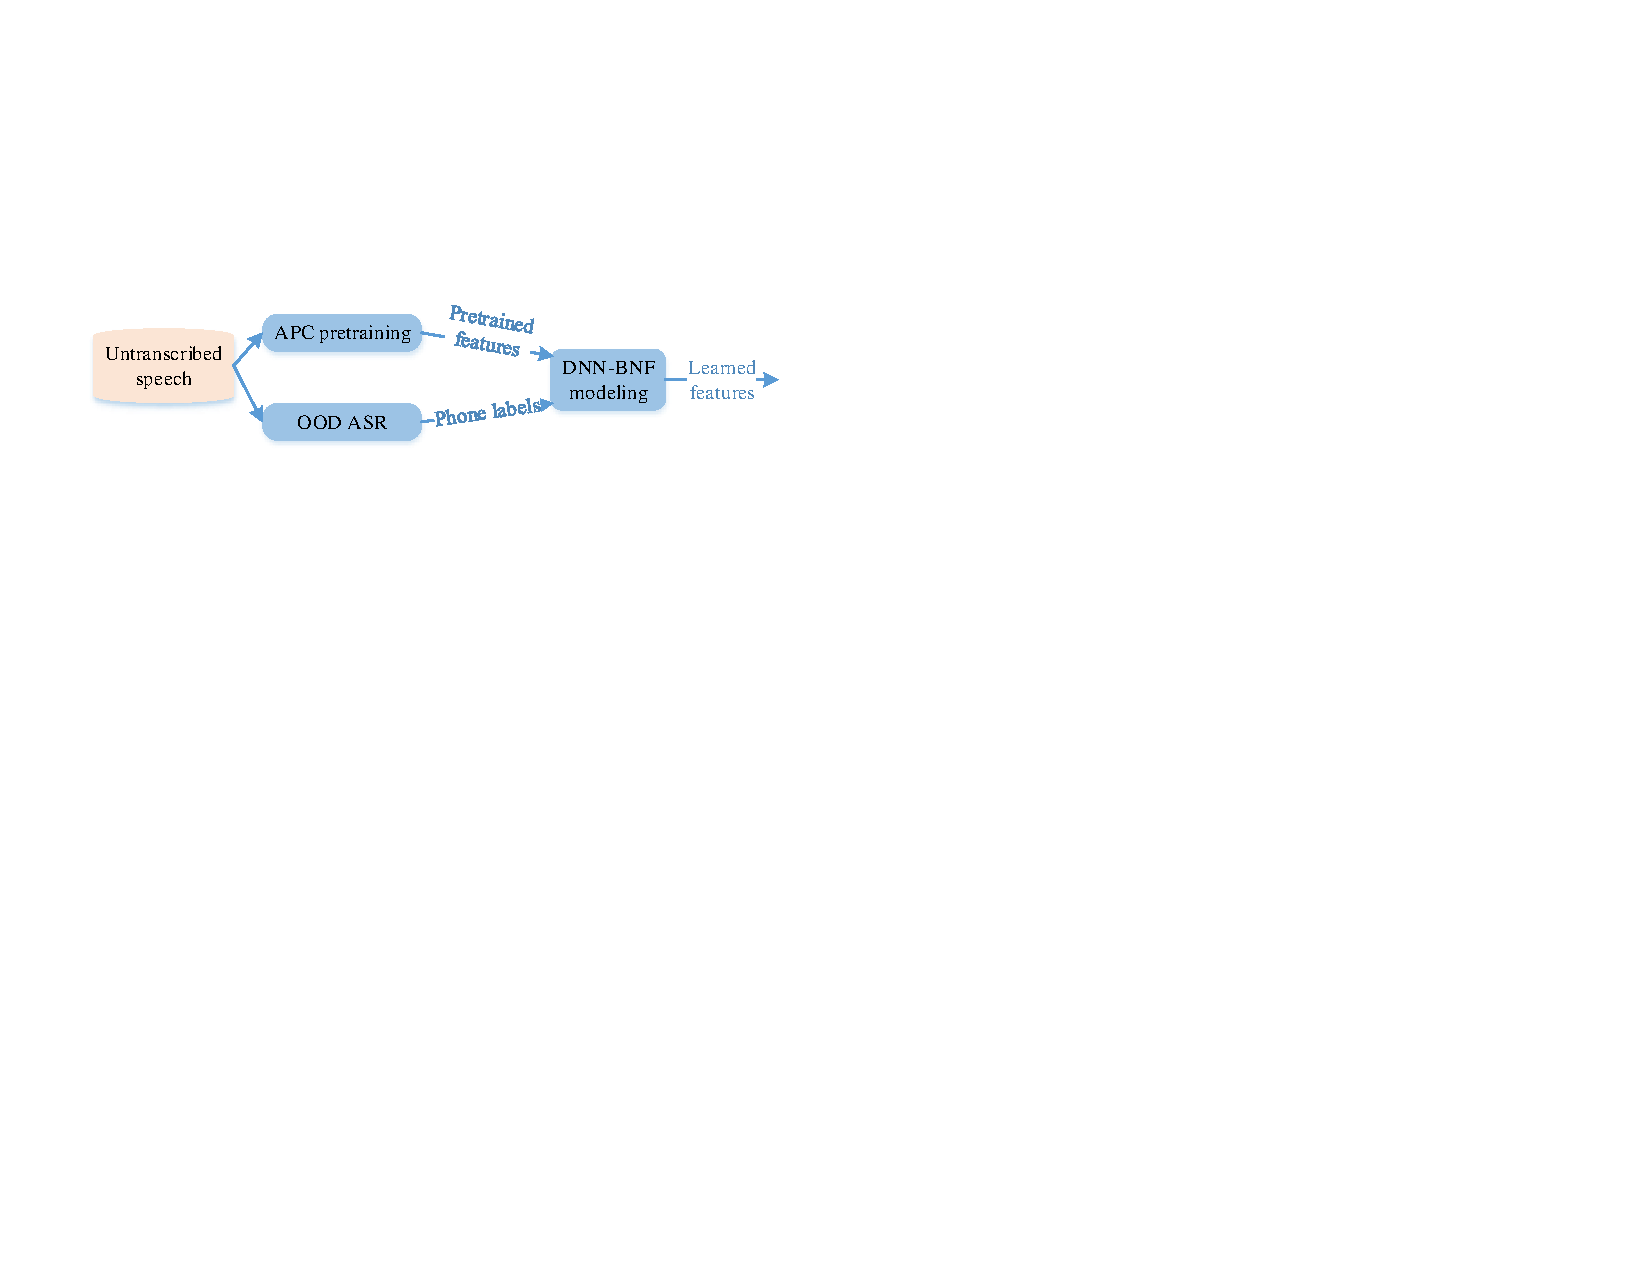
\includegraphics[width=0.95\linewidth]{LaTeX/apc_framework.pdf}
    \caption{General framework of the proposed approaches to unsupervised subword modeling.  }
    \label{fig:general_framework}
\end{figure}
The general framework of our proposed approaches is illustrated in Figure \ref{fig:general_framework}. Given untranscribed speech of a certain  language, the APC  model is used to pretrain the data in an unsupervised manner. An OOD ASR system for a language different from the target language  assigns a phone label to every frame of the data. The APC pretrained features and  cross-lingual phone labels are used to train a DNN-BNF model, with which BNFs are extracted as the subword-discriminative representation.
\subsection{APC pretraining}
APC is an unsupervised generative model proposed for feature representation learning \cite{Chung2019}. 
% It was proposed by \cite{Chung2019} to learn frame-level feature representation which facilitates a wide range of downstream tasks. 
Its effectiveness has been demonstrated in both ASR and SV tasks \cite{Chung2019}. It indicates that APC pretraining preserves both phonetic (subword) and speaker information in original speech,  but are more  separable and are more accessible to task-specific back-end models, comparing to spectral features and other feature learning methods \cite{Chung2019}. 

For our concerned unsupervised subword modeling task, previously adopted feature learning methods 
% such as FHVAE \cite{Feng2019improving} and adversarial training \cite{Higuchi2019} 
are usually designed to suppress speaker variation \cite{Feng2019improving,heck2017feature}. In contrast, the present study applies APC to learn a representation that keeps information in original speech, meanwhile subword information is made more separable to speaker information. The learned representation is expected to facilitate back-end subword-discriminative modeling, and is less risky of losing subword information.


% both subword and speaker information and they are more separable, hence facilitates back-end modeling to learn subword-discriminative representation of speech.%,  %The present study adopts APC to learn a feature representation

Let us assume a certain amount of unlabeled training data $\{\bm{x_1}, \bm{x_2}, \ldots, \bm{x_T}\}$, where $T$ is the total number of frames. At each time step $t$, the encoder of APC model $\textrm{Enc}$ reads as input
$\bm{x_t}$, 
% $\bm{x_{1:t}}=\{\bm{x_1},\ldots,\bm{x_t}\}$ 
and outputs $\bm{y_t}$ (same dimension as $\bm{x_t}$) based on all previous inputs $\bm{x_{1:t}}=\{\bm{x_1},\ldots,\bm{x_t}\}$,
\begin{equation}
    \bm{y_t} = \textrm{Enc} (\bm{x_{1:t}}).
    \label{eqt:enc}
\end{equation}
The goal of APC is to let $\bm{y_t}$ be as close to $\bm{x_{t+n}}$ as possible, where $n$ is a pre-defined constant positive integer. The loss function during APC model training is defined as,
\begin{equation}
    \textrm{Loss} = \sum_{t=1}^{T-n} \left| \bm{y_t} - \bm{x_{t+n}} \right|.
    \label{eqt:apc_loss}
\end{equation}
By minimizing the loss function in Equation (\ref{eqt:apc_loss}), the APC encoder can be trained. Intuitively, increasing $n$ encourages the APC encoder to capture contextual dependencies in speech, 
% more global structures in speech, 
while a small $n$ focuses more on local smoothness.
 
The encoder of APC is realized by the long short-term memory (LSTM) \cite{hochreiter1997long} RNN architecture in this work. Let $L$ denote the number of LSTM layers in the encoder. Equation (\ref{eqt:enc}) is formulated as,
\begin{align}
    \bm{h_0} &= \bm{x_{1:t}},    \\
    \bm{h_l} &= \textrm{LSTM}^l (\bm{h_{l-1}}), l\in \{1,2,\ldots, L\}, \\
    \bm{y_t} &= \bm{W} \bm{h_L}.
\end{align}
Details of the  layer structure $\textrm{LSTM} (\cdot)$ can be seen in \cite{sak2014long}.

After APC training, the output of the top hidden layer $\bm{h_L}$ is extracted as the  learned  representation, and is referred to as \textit{APC features} in this paper. In principle,  $\bm{h_l}$ of any layer $l$ could be used as the learned representation. Results in \cite{Chung2019} suggest that outputs of higher layers  are more suitable for phone classification, while lower layer outputs are  more suitable for speaker classification.
% Here $\bm{h_l}$ denotes the output of  

% , APC pretrained features surpass spectral features 
% which require 
% phonetic and speaker information in APC features are both more accessible to their respective back-end models for ASR and SV tasks.
% (-) Architecture of Enc.\\
% (-) how to extract features from APC to back-end.
% APC pretrained features  tend to retain as much information encoded in original speech representation as  possible. 
% different types of information in APC features, such as phonetic and speaker information, are both more accessible to the back-end models corresponding to their respective tasks.
\subsection{Cross-lingual phone-aware DNN-BNF}
% The back-end of our proposed approaches is t
The DNN-BNF model  \cite{chen2017multilingual,feng2018exploiting} is adopted as the back-end of our proposed approaches. It is a DNN with a low-dimension hidden (BN) layer in the middle. BNFs are known of providing compact yet subword-discriminative representation of speech \cite{grezl2009investigation}.  
% Training of a subword-discriminative DNN-BNF model requires frame labels \cite{chen2017multilingual}. 
Under the zero-resource scenario, phonetic alignments of target speech required for DNN-BNF modeling cannot be obtained due to the absence of transcriptions. 

This study leverages an OOD language-mismatched ASR system to generate cross-lingual phonetic alignments for in-domain speech.
Specifically, the OOD ASR is used to decode  and find the best paths for every in-domain speech utterances, as was done in \cite{feng2019_TASLP}. Through decoding, each speech frame is assigned with a triphone HMM state modeled by the OOD ASR. These labels provide phonetic representation for the target speech from a cross-lingual perspective. Although languages vary greatly in pronunciation, speech sounds in different languages are believed to have much overlap at phoneme level.
It is worth noting that decoding results depend on the relative weighting  of the ASR AM and language model (LM). In this study, the LM carries a very small weight, in order to ensure decoding results mainly reflect acoustic characteristics of target speech.

After obtaining cross-lingual triphone HMM state labels, a DNN-BNF model is trained with target speech, using these labels as supervision.  
The DNN-BNF is trained to optimize cross-lingual phone classification accuracy.
The inputs to DNN-BNF are APC features. 
After training, the DNN-BNF is used to extract BNFs for target speech as the subword-discriminative feature representation. 
% XXX cross-lingual phone-aware manner.

The choice of language identities of OOD ASR systems is flexible in principle. In the present study, a comparison is made by applying OOD ASR systems from different languages to generate cross-lingual labels, in order to study the influence of selecting OOD ASRs on final performance.
% its influence towards the final performance.
% our proposed approaches.

% (-) OOD ASR decoding\\
% (-) DNN-BNF training with APC features and cross-lingual phone labels\\
% (-) Effect of OOD language identity.
% Authors should observe the following rules for page layout. A highly recommended way to meet these requirements is to use a given template (Microsoft Word?? or LaTeX) and check details against the corresponding example PDF file. Given templates, Microsoft Word\textregistered\ or \LaTeX, can be adapted/imported easily in other software such as LibreOffice, Apple Pages, Lua\LaTeX, and Xe\LaTeX, but please be careful to match the layout of the provided PDF example.

\section{Experimental setup}

\subsection{Database and evaluation metric}
Experiments in this study are carried out on two databases: Libri-light \cite{kahn2019librilight} and ZeroSpeech 2017 \cite{Dunbar2019}. Libri-light is a newly published   database to facilitate research on ASR under limited or zero resource scenarios. It is by far the largest public database to support evaluation on unsupervised subword modeling. The language in Libri-light is English. The \texttt{unlab-600} set from Libri-light is adopted as training data in most of our experiments. This set contains $36,229$ utterances by $489$ speakers, summing up to $526$ hours. In addition, we randomly select subsets of utterances in \texttt{unlab-600}  to form smaller-sized training data. There are four smaller-sized training sets constructed in this study, with the numbers of utterances ranging from $900$ to $3.6$K, $7.2$K and $14.4$K. Details of \texttt{unlab-600} and the training subsets are summarized in Table \ref{tab:libri_light_data}.
\begin{table}[htbp]
\renewcommand\arraystretch{0.90}
\centering
\caption{Libri-light training data and its subsets.}
\resizebox{1 \linewidth}{!}{%
\begin{tabular}{l|ccccc}      
% \hline      
% \toprule
& Unlab-600 & Sub14.4K & Sub7.2K & Sub3.6K & Sub0.9K \\
%  & \multicolumn{3}{c|}{ Training} & Test \\
\midrule
\# Utterances & $36,229$ & $14,400$ &$7,200$ &$3,600$ &$900$ \\
\# Speakers & $489$ & $438$ & $393$ & $351$ & $244$ \\
\# Hours &$526$& $209$ & $104$ & $52$ & $13$ \\
%  & Duration  &\#speakers-R\tablefootnote{``speakers-R/-L'' denotes speakers with rich/limited speech data.} &\#speakers-L\footnotemark[1]  & Duration\\
% \hline
% \midrule

% Training hours:  & $19.3$ & $81.5$ & $105.3$ \\
% Test hours:& $0.6$ & $0.7$ & $5.9$ \\
% Basic acoustic unit:  & Phone & Phone & Initial-Final \\
% \#basic units (inc. sil):& $33$ & $87$ & $61$ \\
% \#tied CD-HMM states:& $2462$ & $3431$ & $2386$ \\ 
% Lexicon size:& $ $ & $ 133K$& $ $ \\
% $\#$ Phonemes: &$43$& $46$&$ 29$& $44$& $38$\\
% \hline
% \bottomrule
\end{tabular}%
% \footnotetext{`speakers-R/-L' denotes speakers with rich/limited speech data}
}
\label{tab:libri_light_data}
\end{table}

The evaluation data in Libri-light consists of four sets, \texttt{dev-clean, dev-other, test-clean} and \texttt{test-other}. They are the same as that of Librispeech corpus \cite{panayotov2015librispeech}.


ZeroSpeech 2017 database is also used in our experiments, but only for performance evaluation.  English test set is adopted. 
% contains three languages, English, French and Mandarin. In our experiments, ZeroSpeech training data is not used, and 
% Our systems are trained solely on Libri-light. ZeroSpeech evaluation data for English is used. 
It is organized into subsets of differing utterance lengths (1s, 10s and 120s).
% consists of three utterance length settings, $1$s
% English 


The evaluation metric is ABX subword discriminability.
The ABX task is to decide whether $X$ belongs to $x$ or $y$ if $A$ belongs to $x$ and $B$ belongs to $y$, where $A$, $B$ and $X$ are three speech segments, $x$ and $y$ are two phonemes that differ in the central sound (e.g., \quotes{beg}-\quotes{bag}). 
Each pair of $A$ and $B$ are generated by the same speaker. 
ABX error rates for \textit{within-speaker} and \textit{across-speaker} are evaluated separately, depending on whether $X$ and $A(B)$ belong to the same speaker. 
\subsection{APC setup}
\subsection{OOD ASR systems}
\subsection{DNN-BNF setup}
\section{Results and discussion}
% \section{Discussion}

This is the discussion. This is the discussion. This is the discussion. Is there any discussion?


\section{Conclusions}


\section{Acknowledgements}




\bibliographystyle{IEEEtran}

\bibliography{mybib}

% \begin{thebibliography}{9}
% \bibitem[1]{Davis80-COP}
%   S.\ B.\ Davis and P.\ Mermelstein,
%   ``Comparison of parametric representation for monosyllabic word recognition in continuously spoken sentences,''
%   \textit{IEEE Transactions on Acoustics, Speech and Signal Processing}, vol.~28, no.~4, pp.~357--366, 1980.
% \bibitem[2]{Rabiner89-ATO}
%   L.\ R.\ Rabiner,
%   ``A tutorial on hidden Markov models and selected applications in speech recognition,''
%   \textit{Proceedings of the IEEE}, vol.~77, no.~2, pp.~257-286, 1989.
% \bibitem[3]{Hastie09-TEO}
%   T.\ Hastie, R.\ Tibshirani, and J.\ Friedman,
%   \textit{The Elements of Statistical Learning -- Data Mining, Inference, and Prediction}.
%   New York: Springer, 2009.
% \bibitem[4]{YourName17-XXX}
%   F.\ Lastname1, F.\ Lastname2, and F.\ Lastname3,
%   ``Title of your INTERSPEECH 2020 publication,''
%   in \textit{Interspeech 2020 -- 20\textsuperscript{th} Annual Conference of the International Speech Communication Association, September 15-19, Graz, Austria, Proceedings, Proceedings}, 2020, pp.~100--104.
% \end{thebibliography}

\end{document}
